\documentclass[10pt,twocolumn,letterpaper]{article}
\usepackage[T1]{fontenc}
\usepackage{newtxtext,newtxmath}
\usepackage[letterpaper,top=1in,bottom=1in,left=0.75in,right=0.75in,columnsep=0.3125in]{geometry}
\usepackage{graphicx,booktabs,amsmath,multirow,xcolor,microtype,enumitem}
\usepackage[font=small,labelfont=bf,skip=4pt]{caption}
\usepackage[colorlinks=true,linkcolor=blue!50!black,citecolor=blue!50!black,urlcolor=blue!50!black]{hyperref}
\usepackage[capitalise,noabbrev]{cleveref}
\usepackage{tikz}
\usetikzlibrary{positioning,arrows.meta,calc}
\graphicspath{{figs/}}
\setlist{itemsep=1pt,topsep=2pt,leftmargin=1.2em}
\newcommand{\pts}{\,pts}
\newcommand{\etal}{et~al.}
\newcommand{\OKS}{\mathrm{OKS}}
\definecolor{acc}{HTML}{2A78D6}\definecolor{org}{HTML}{EB6834}

\title{\Large\bf One Prediction per Person: What the Confidence Score\\ Is Worth for Keypoint AP on Unseen Cameras}
\author{Anonymous authors\\ UPAR Challenge 2027, Track 3 technical report}
\date{}

\begin{document}
\maketitle

\begin{abstract}
When person boxes are given, a top-down pose estimator makes exactly one prediction per person, and COCO keypoint AP then depends on two things: how accurate each prediction is, and how well the confidence score orders the predictions. We show that in this regime AP at each OKS threshold lies between $f_t^2$ and $f_t$, where $f_t$ is the fraction of correct predictions, and that the two bounds match the AP of an uninformative and a perfect score on our data. We measure both factors on UPAR 2027 Track~3 with ViTPose++ models evaluated on held-out datasets. With the keypoints fixed, a perfect score would add 1.3--1.5 points of AP, more than averaging the heatmaps of a second model (0.1--0.5 points). Most of this value lies in separating excellent predictions from good ones, at OKS 0.95, rather than in demoting failures. The usual score, the mean of the heatmap maxima, includes the two ear channels, which this keypoint format never annotates. Removing them recovers most of what a gradient-boosted rescorer on heatmap statistics achieves, and the rescorer itself, validated across held-out datasets at both levels, recovers 12--30\% of the oracle's gain. On the hidden test it added 0.15 points, within its held-out range. Two further measurements change the picture of where the errors are. Fine-tuning appears to be worth 23 points, but on the joints that COCO and PoseTrack share it is worth 0.7, so most of that gain is learning a head-keypoint definition. And left--right inversions affect only 1.3\% of PETA people, yet fixing them would add 1.65 points, more than a perfect score. The system scored 0.8992 AP on the hidden test, against 0.8813 for a fine-tuned ViTPose++ base model.
\end{abstract}

%=====================================================================
\section{Introduction}

Top-down pose estimation finds people with a detector and then predicts their joints inside each box~\cite{simplebaseline,hrnet,vitpose}. Track~3 of the UPAR 2027 challenge supplies the person boxes and asks for 17 PoseTrack18 keypoints on low-resolution surveillance crops from cameras that are absent from training. Since the boxes are given, every person receives exactly one prediction.

That fact changes what the metric rewards. COCO keypoint AP sorts all predictions by their confidence score and integrates precision over recall at ten OKS thresholds~\cite{coco}. In multi-person settings the score mostly decides which of several candidate poses counts; here it only decides the order in which a fixed set of predictions is visited. A score that orders them perfectly and one that orders them randomly produce different AP from identical keypoints. How large that difference is, and where it arises, determines whether effort should go into better keypoints or into a better score.

This report measures it, designs a score around the measurement, and asks where the remaining errors are. Our contributions are:
\begin{itemize}
\item An analysis of AP in the one-prediction-per-box regime, with bounds $f_t^2$ and $f_t$ that we validate on held-out data (\cref{sec:task}).
\item A measurement of the score's value per dataset and per threshold, and a decomposition showing that it lies mainly in ordering good predictions, not in demoting failures (\cref{sec:score}).
\item A learned rescorer validated by leave-one-dataset-out at two levels, together with the finding that excluding the never-annotated ear channels from the default score already captures most of its gain (\cref{sec:rescore}).
\item Two corrections to the usual reading of such systems: most of the gain from fine-tuning is a keypoint-definition effect, and left--right inversions cost more AP than the entire score gap on one dataset (\cref{sec:models,sec:errors}).
\end{itemize}

%=====================================================================
\section{Related Work}

\paragraph{Top-down pose estimation.} SimpleBaseline~\cite{simplebaseline} and HRNet~\cite{hrnet} predict one heatmap per joint. ViTPose~\cite{vitpose} uses a plain vision transformer initialized with MAE~\cite{mae}, and ViTPose++~\cite{vitposepp} trains it on several pose datasets with dataset-specific expert layers. UDP~\cite{udp} and DARK~\cite{dark} remove biases in coordinate transforms and decoding. We use these components unchanged.

\paragraph{Error diagnosis and scoring.} Ronchi and Perona~\cite{ronchi} decompose keypoint errors into jitter, inversion (left and right confused within a person), swap (joints of another person) and miss, and measure the AP lost to suboptimal scores with an oracle. We adopt their terms. Our setting differs in having exactly one prediction per box, which makes the score's effect analyzable in closed form, and in evaluating on unseen domains.

\paragraph{Learned rescoring.} Papandreou~\etal~\cite{gpose} score a person by heatmap maxima. DEKR~\cite{dekr} trains a small network on predicted keypoints to estimate OKS, and CCNet~\cite{ccnet} predicts OKS from internal features of the pose network. Our rescorer uses only statistics of the output heatmaps, so it runs outside a packaged model, and we validate it on held-out datasets rather than on the training distribution.

\paragraph{Domain adaptation for pose.} RegDA~\cite{regda} and the unified framework of Kim~\etal~\cite{kim2022} adapt keypoint detectors with unlabeled target images. The challenge forbids using test images, so we rely on leave-one-dataset-out evaluation instead.

%=====================================================================
\section{Task, Metric and the One-Prediction Regime}
\label{sec:task}

\paragraph{Data.} Each training sample is an image with one person box and 17 PoseTrack18 keypoints~\cite{posetrack}. The two ear slots are never annotated and never scored. Labels cover 42{,}736 people from three UPAR datasets: PA100k (19{,}499), Market1501 (12{,}923) and PETA (10{,}314). The hidden test set has 30{,}245 boxes from an unseen camera domain, some in images with several boxes.

\paragraph{OKS and AP.} The object keypoint similarity of a prediction $\hat x$ with ground truth $x$ is
\begin{equation}
\OKS=\frac{\sum_k\exp\!\big(-\|\hat x_k-x_k\|^2/2s^2\kappa_k^2\big)\,\mathbb 1[v_k>0]}{\sum_k\mathbb 1[v_k>0]},
\end{equation}
where $s^2$ is the person's area, $\kappa_k$ a per-joint constant and $v_k$ the visibility label. The PoseTrack head points use the COCO eye constant $\kappa=0.025$, the smallest of all joints. At threshold $t$ a prediction is correct if $\OKS>t$. Predictions are sorted by score, AP is the area under the precision--recall curve, and the final metric averages AP over $t\in\{0.50,0.55,\ldots,0.95\}$~\cite{coco}. We report differences in points (pts), where 1\pts{} is 0.01 AP.

\paragraph{AP with one prediction per box.} Let $f_t$ be the fraction of predictions that are correct at threshold $t$. If the score orders predictions perfectly, all correct ones come first, precision is 1 until recall reaches its maximum $f_t$, and AP equals $f_t$. If the score carries no information, precision stays near $f_t$ at every depth and AP is about $f_t^2$. For $f_t=0.8$ the two differ by 16 points with identical keypoints. \Cref{tab:bounds} checks the bounds on held-out data. The mean of $f_t^2$ is within half a point of the AP of a constant score on all three datasets. The mean of $f_t$ exceeds the oracle AP by about 0.5\pts, the cost of COCO's 101-point interpolation. The bounds also show where the score can matter: $f_t$ is at least 0.95 for all thresholds up to 0.85, and falls to 0.69--0.76 at 0.95.

\begin{table}[t]
\centering\small
\setlength{\tabcolsep}{3.5pt}
\resizebox{\columnwidth}{!}{%
\begin{tabular}{@{}lccc@{}}
\toprule
Held-out dataset & PETA & PA100k & Market \\
\midrule
$f_{0.50}$ / $f_{0.85}$ / $f_{0.95}$ & .991 / .950 / .759 & .990 / .961 / .690 & .998 / .972 / .705 \\
mean of $f_t^2$ & 90.41 & 90.33 & 92.41 \\
AP, constant score & 90.50 & 90.06 & 92.00 \\
mean of $f_t$ & 94.85 & 94.64 & 95.74 \\
AP, oracle score (true OKS) & 94.36 & 94.26 & 95.25 \\
\bottomrule
\end{tabular}}
\caption{The one-prediction bounds against measured AP (fine-tuned ViTPose++ huge, keypoints fixed; AP $\times100$).}
\label{tab:bounds}
\end{table}

\paragraph{Rules.} The challenge allows pretraining on COCO and PoseTrack18 only. ViTPose++ checkpoints are trained on several pose datasets and initialized from MAE on ImageNet. We use them because the organizers' official example submission is built on a ViTPose++ checkpoint, which we read as permitting this model family. Test images are not used for training, pseudo-labeling or tuning.

%=====================================================================
\section{Keypoint Model and Protocol}
\label{sec:method}

\begin{figure*}[t]
\centering
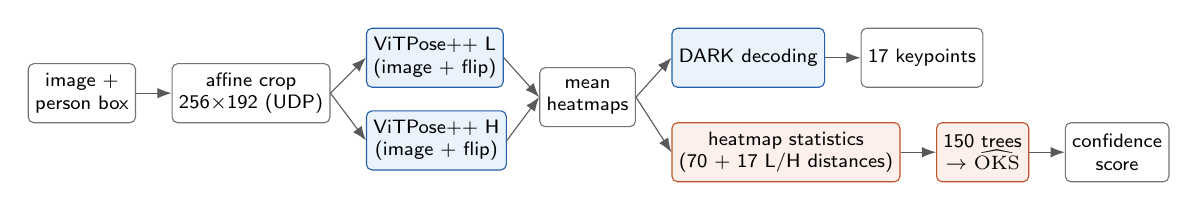
\begin{tikzpicture}[font=\sffamily\scriptsize, node distance=3.5mm and 4.5mm,
  box/.style={draw=black!55, rounded corners=2pt, fill=white, align=center, minimum height=7.5mm, inner sep=2.5pt},
  hl/.style={box, fill=acc!10, draw=acc!80!black}, tc/.style={box, fill=org!10, draw=org!80!black},
  arr/.style={-{Latex[length=1.8mm]}, black!65}]
\node[box] (img) {image +\\ person box};
\node[box, right=of img] (crop) {affine crop\\ 256$\times$192 (UDP)};
\node[hl, right=of crop, yshift=4.5mm] (l) {ViTPose++ L\\ (image + flip)};
\node[hl, right=of crop, yshift=-6mm] (h) {ViTPose++ H\\ (image + flip)};
\node[box, right=of l, yshift=-5mm] (avg) {mean\\ heatmaps};
\node[hl, right=of avg, yshift=5mm] (dark) {DARK decoding};
\node[box, right=of dark] (kp) {17 keypoints};
\node[tc, right=of avg, yshift=-7mm] (feat) {heatmap statistics\\ (70 + 17 L/H distances)};
\node[tc, right=of feat] (gbm) {150 trees\\ $\to\widehat{\OKS}$};
\node[box, right=of gbm] (sc) {confidence\\ score};
\draw[arr] (img)--(crop); \draw[arr] (crop.east)--(l.west); \draw[arr] (crop.east)--(h.west);
\draw[arr] (l.east)--(avg.west); \draw[arr] (h.east)--(avg.west); \draw[arr] (avg.east)--(dark.west);
\draw[arr] (avg.east)--(feat.west); \draw[arr] (dark)--(kp); \draw[arr] (feat)--(gbm); \draw[arr] (gbm)--(sc);
\end{tikzpicture}
\caption{Submitted system. The blue path produces the keypoints; the orange path only replaces the confidence score.}
\label{fig:pipe}
\end{figure*}

\paragraph{Model.} \Cref{fig:pipe} shows the system. ViTPose++~\cite{vitposepp} (whose public checkpoints are named ViTPose+) encodes a $256\times192$ crop as $16\times12$ tokens and decodes 17 heatmaps of $64\times48$. We use the COCO expert index. COCO and PoseTrack18 share the nose and the 12 body joints and differ at the head: PoseTrack's head-bottom and head-top replace COCO's eyes. Each box is extended to a 3:4 aspect ratio, enlarged by 1.25, and warped with the pixel-center convention of UDP~\cite{udp}.

\paragraph{Training.} Targets are Gaussian heatmaps with $\sigma=2$ cells and the loss is the visibility-weighted mean squared error. Augmentation uses scale jitter in $[0.75,1.25]$, shifts up to 8\%, rotations drawn from a Gaussian with $\sigma=30^\circ$ clipped at $\pm40^\circ$ (probability 0.4), flips with left--right swapping, and brightness and contrast jitter. We train with AdamW, learning rate $5\cdot10^{-5}$, layer decay 0.75 and batch 64.

\paragraph{Inference.} Each crop runs twice, once flipped; the flipped heatmaps are flipped back with left and right channels swapped and averaged with the original. For the ensemble, the heatmaps of the large and huge models are averaged before DARK decoding~\cite{dark}.

\paragraph{Protocol and noise.} We train on two datasets for two epochs and evaluate on every labeled person of the third (leave-one-dataset-out). Submitted models train for five epochs on all three. Each configuration was trained once, so training noise must be bounded indirectly: the held-out AP of one model moves by up to 0.35\pts\ between consecutive epochs (ViTPose++ base on PETA: 93.23, 92.97, 93.32 after epochs 1--3). Comparisons of scores are different. They keep the keypoints fixed, so training noise cancels, and the remaining uncertainty is the sampling of people, which we estimate by bootstrap.

%=====================================================================
\section{Keypoint Results}
\label{sec:models}

\paragraph{What fine-tuning buys.} Without fine-tuning, ViTPose++ huge reaches only 70.2 AP on held-out PETA, against 93.0 after two epochs on the other datasets (\cref{tab:lodo}). This gap is not mainly a domain gap. The COCO model's eye channels are scored as PoseTrack head points, with the smallest $\kappa$. Its AP50 is already 97.7, so it finds the people and loses at strict thresholds, as a systematic offset would. Scoring both models on the 13 shared joints only (the PoseTrack head points removed from the ground truth) shrinks the gap to 0.66\pts: 92.97 zero-shot against 93.63 fine-tuned. Most of the 23-point gain is therefore the network learning PoseTrack's head-keypoint definition and annotation convention. Appearance adaptation to low-resolution surveillance accounts for less than one point, and it appears at the strictest thresholds: on shared joints the zero-shot model is slightly better at AP50 and AP75 (97.74 and 96.58 against 97.41 and 96.28).

\begin{table}[t]
\centering\small
\setlength{\tabcolsep}{3.2pt}
\resizebox{\columnwidth}{!}{%
\begin{tabular}{@{}lcccc@{}}
\toprule
Held-out dataset & PETA & PA100k & Market & Mean \\
\midrule
Huge, zero-shot & 70.25 & 70.18 & 69.95 & 70.13 \\
Huge, zero-shot, shared joints & 92.97 & -- & -- & -- \\
Huge, fine-tuned, shared joints & 93.63 & -- & -- & -- \\
\midrule
Large, fine-tuned & 93.14 & 92.44 & 93.92 & 93.17 \\
Huge, fine-tuned & 93.04 & 92.81 & 93.96 & 93.27 \\
Large + huge & 93.52 & 92.91 & 94.16 & 93.53 \\
Large + huge + learned score & 93.77 & 92.97 & 94.31 & 93.68 \\
\bottomrule
\end{tabular}}
\caption{OKS AP ($\times100$) on held-out datasets, two epochs of fine-tuning on the other two. ``Shared joints'' removes the PoseTrack head points from the ground truth; it was measured on PETA only.}
\label{tab:lodo}
\end{table}

\paragraph{Model size and ensembling.} Large and huge differ by $-0.10$, $+0.37$ and $+0.04$\pts\ on the three held-out datasets, inside the epoch-to-epoch variation on two of them. Averaging their heatmaps improves every dataset, by 0.48, 0.10 and 0.20\pts\ over huge alone, but only the PETA gain clearly exceeds that variation. We therefore treat both choices as weakly supported by the protocol; the hidden test agrees in sign with both (\cref{sec:test}). An ensemble of two networks is also the most expensive change in this report, which motivates asking what the score is worth by comparison.

%=====================================================================
\section{How Much Is the Score Worth, and Where?}
\label{sec:score}

\begin{table}[t]
\centering\small
\setlength{\tabcolsep}{3.2pt}
\resizebox{\columnwidth}{!}{%
\begin{tabular}{@{}lcccc@{}}
\toprule
Confidence score & PETA & PA100k & Market & Mean \\
\midrule
Constant & 90.50 & 90.06 & 92.00 & 90.86 \\
Mean of 17 heatmap maxima (default) & 93.04 & 92.81 & 93.96 & 93.27 \\
Default, failures moved last (oracle) & 93.43 & 92.89 & 94.01 & 93.44 \\
Mean of 15 maxima, ears excluded & 93.39 & 92.96 & 94.14 & 93.50 \\
Learned (\cref{sec:rescore}) & 93.44 & 92.99 & 94.15 & 93.53 \\
True OKS (oracle) & 94.36 & 94.26 & 95.25 & 94.62 \\
\bottomrule
\end{tabular}}
\caption{OKS AP ($\times100$) with the keypoints of the held-out huge models fixed and different scores. ``Failures moved last'' keeps the default order but places every prediction with OKS $<0.5$ at the end.}
\label{tab:choices}
\end{table}

\Cref{tab:choices} holds the keypoints of the held-out huge models fixed and varies only the score. The default score is worth 2.4\pts\ over a constant one, and a perfect score would add another 1.32, 1.45 and 1.29\pts\ on the three datasets. That is larger than the ensemble gain of \cref{sec:models}, at no cost in keypoint quality. The default score is only moderately related to accuracy: its Spearman correlation with OKS is 0.52 on PETA, 0.36 on PA100k and 0.44 on Market1501.

\paragraph{Failures are not where the value is.} An intuitive reason for a poor score is that the network is confident on the wrong person or the wrong side of the body, and \cref{fig:examples} shows such a case. But an oracle that only moves every prediction with OKS below 0.5 to the end of the list gains 0.39, 0.08 and 0.05\pts, a small fraction of the full oracle. Failures are too rare to matter much: at most 1\% of predictions are below OKS 0.5 on any dataset.

\begin{figure*}[t]
\centering
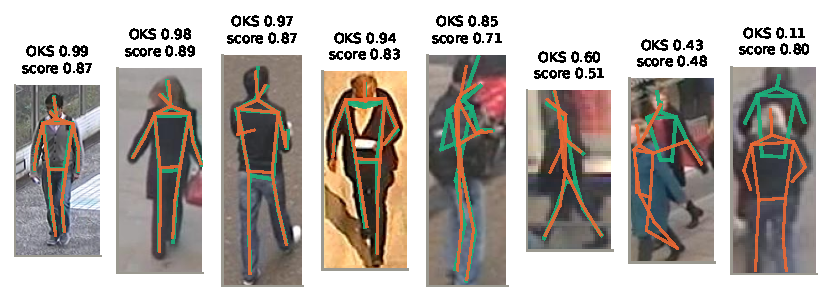
\includegraphics[width=\linewidth]{examples.pdf}
\caption{Ground truth (green) and predictions of the PETA-held-out huge model (orange), from high to low OKS, with the default score. The last crop is a confident prediction on the person in front.}
\label{fig:examples}
\end{figure*}

\paragraph{The value lies at the strictest threshold.} \Cref{fig:thr} splits the oracle's gain by threshold. On PA100k and Market1501, 79\% and 78\% of it comes from OKS 0.95, the one threshold at which a quarter or more of predictions fail. On PETA the oracle's gain is spread more evenly, with 47\% at 0.95. For the median PETA person (box height 149 pixels), a per-joint similarity of 0.95 on a shoulder allows an error of about 5 pixels, under two cells of the $64\times48$ heatmap. A useful score must therefore separate excellent predictions from good ones, a much finer task than flagging failures.

\begin{figure*}[t]
\centering
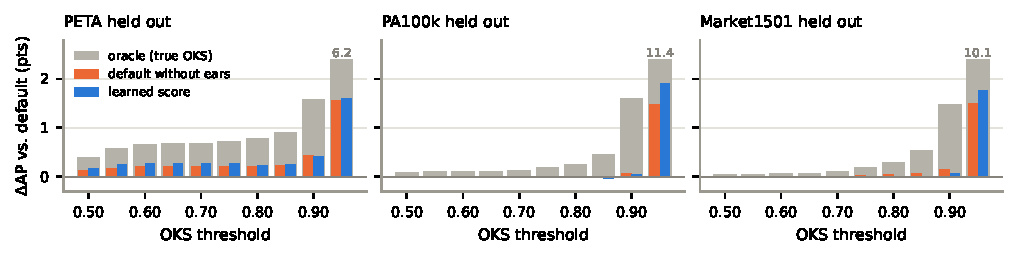
\includegraphics[width=\linewidth]{per_threshold.pdf}
\caption{AP gain over the default score at each OKS threshold, per held-out dataset (huge model, keypoints fixed). Grey: true OKS as score (clipped; values printed). Orange: default score without the ear channels. Blue: learned score. AP is the mean of the ten thresholds, so a gain of 1.6 at one threshold adds 0.16\pts.}
\label{fig:thr}
\end{figure*}

%=====================================================================
\section{Learning the Score}
\label{sec:rescore}

\paragraph{Design.} The score should rank predictions by their true OKS, use only the outputs of the pose network so that the network stays unchanged, and be validated on domains it was not trained on. We describe each person by 70 statistics of the averaged heatmaps: the 17 maxima; for each joint, the distance between the peaks decoded from the original and the flipped image; for each joint, the ratio of total non-negative heatmap mass to the peak, which grows for wide or multi-peak heatmaps; for each joint, the spatial standard deviation; and the log box area and aspect ratio. With two models we add the 17 distances between their peaks. The target is the true OKS. We use histogram gradient boosting~\cite{friedman,lightgbm} with 150 trees of at most 7 leaves, learning rate 0.05 and at least 100 samples per leaf.

\paragraph{Two-level protocol.} The features of each dataset come from pose models that never saw it, and the regressor is trained on the other two datasets and tested on it. The submitted regressor is refit on all three. The tree size was chosen after a first configuration (15 leaves, 300 trees) on the same folds, so the reported numbers carry a small selection effect; the two configurations differ by 0.03\pts\ on average.

\begin{table}[t]
\centering\small
\setlength{\tabcolsep}{3.2pt}
\resizebox{\columnwidth}{!}{%
\begin{tabular}{@{}lcccc@{}}
\toprule
Rescorer (huge, held out) & PETA & PA100k & Market & Mean \\
\midrule
Default score & 93.04 & 92.81 & 93.96 & 93.27 \\
MLP, one hidden layer & 92.66 & 92.52 & 93.68 & 92.95 \\
Ridge, all features & 93.11 & 92.99 & 94.13 & 93.41 \\
Ridge, maxima + flip & 93.28 & 92.97 & 94.11 & 93.45 \\
Boosting, 15 leaves, 300 trees & 93.38 & 92.93 & 94.15 & 93.49 \\
Boosting, submitted & 93.44 & 92.99 & 94.15 & 93.53 \\
\midrule
\multicolumn{5}{@{}l}{\emph{Submitted boosting without one feature family}} \\
without maxima & 93.39 & 92.97 & 94.09 & 93.48 \\
without flip distances & 93.43 & 92.97 & 94.15 & 93.52 \\
without mass/peak & 93.44 & 93.00 & 94.15 & 93.53 \\
without spread & 93.45 & 92.98 & 94.15 & 93.53 \\
without box size & 93.43 & 92.98 & 94.16 & 93.52 \\
\bottomrule
\end{tabular}}
\caption{Rescorers trained on two datasets and tested on the third (AP $\times100$). Lower block: refits without one feature family.}
\label{tab:rescore}
\end{table}

\paragraph{Results.} \Cref{tab:rescore} shows that boosting improves all three held-out datasets, by 0.40, 0.18 and 0.19\pts. Bootstrapping people with the models fixed gives standard errors of 0.05, 0.03 and 0.02\pts\ for these gains, so they are well above sampling noise. They recover 30\%, 12\% and 15\% of the oracle's gain. Rank correlation with OKS rises from 0.52 to 0.63 on PETA, from 0.36 to 0.43 on PA100k and from 0.44 to 0.48 on Market1501. The MLP falls below the default score on all three; it was not tuned, so we draw no conclusion from it. Removing any one feature family changes the mean by at most 0.05\pts, so the features are largely redundant. In particular, the box-size features do not act as a dataset identifier, a concern because all Market1501 crops have the same size. On the ensemble, the rescorer adds 0.25, 0.06 and 0.15\pts\ (\cref{tab:lodo}).

\paragraph{Most of the gain is a fix to the default score.} The default score averages the maxima of all 17 heatmap channels, including the two ear channels, which PoseTrack never annotates and the metric never scores. Their confidence says nothing about the scored joints. Simply averaging the other 15 maxima gains 0.35, 0.15 and 0.18\pts\ (\cref{tab:choices}), most of the rescorer's gain, and leaves the learned score ahead by only 0.05, 0.03 and 0.01\pts, about two standard errors or less (each 0.02\pts). \Cref{fig:thr} shows the two following each other threshold by threshold. Other simple formulas evaluated on the same held-out features, such as the geometric mean, the minimum or a $\kappa$-weighted mean, do no better than the default. The learned score's advantage is therefore not the trees; it is mainly that the boosting learned to ignore the unscored channels.

\paragraph{Where the learned gain is.} On PA100k and Market1501 essentially all of the learned gain is at OKS 0.95, and on PA100k it is slightly negative at every threshold up to 0.85 (\cref{fig:thr}). On PETA it is spread over all thresholds, with about 40\% at 0.95. PETA is also the dataset with the most inversions (\cref{sec:errors}), which a score can demote at every threshold, consistent with its larger failure oracle in \cref{tab:choices}.

%=====================================================================
\section{Where the Remaining Errors Are}
\label{sec:errors}

\paragraph{Inversions.} Some predictions with OKS below 0.5 still receive high scores, and drawn on the image their skeletons look plausible. Swapping left and right in the prediction tests whether they are inversions in the sense of Ronchi and Perona~\cite{ronchi}. \Cref{tab:swap} shows that on PETA and Market1501 more than half of the predictions below OKS 0.5 exceed 0.8 after the swap, and on PA100k 29\% do. Inversions are rare: a swap improves OKS by more than 0.2 for 1.3\%, 0.6\% and 0.2\% of people. But replacing those predictions by their swapped versions, with the default score, raises AP by 1.65\pts\ on PETA, more than the entire score oracle there, and by 0.42 and 0.04\pts\ on the other two datasets. They are hard to detect from heatmaps because the network is confident about where the joints are. Flip testing cannot reveal them either: flipping an image does not change whether the person faces the camera, so a facing-direction error is made consistently on both passes and the flip-disagreement feature stays low. We have not checked how many of these cases are annotation errors, which at this resolution are possible.

\begin{table}[t]
\centering\small
\setlength{\tabcolsep}{3.5pt}
\resizebox{\columnwidth}{!}{%
\begin{tabular}{@{}lccc@{}}
\toprule
& PETA & PA100k & Market \\
\midrule
Predictions with OKS $<0.5$ & 97 & 187 & 21 \\
\quad of which OKS $>0.8$ after left--right swap & 51 & 55 & 12 \\
People whose OKS rises by $>0.2$ after swap & 1.3\% & 0.6\% & 0.2\% \\
AP, default score & 93.04 & 92.81 & 93.96 \\
AP, inversions fixed, default score & 94.69 & 93.23 & 94.00 \\
AP, inversions fixed, oracle score & 95.45 & 94.65 & 95.25 \\
\bottomrule
\end{tabular}}
\caption{Left--right inversions of the held-out huge models and the AP they cost.}
\label{tab:swap}
\end{table}

\paragraph{Joints and person size.} \Cref{fig:joints} shows the per-joint loss of keypoint similarity. The three head points are worst, with three to five times the loss of shoulders and hips. Part of this is the metric, since they have the smallest $\kappa$, and part is that head-bottom and head-top are defined by convention rather than anatomy. Smaller people are harder: on PETA the smallest fifth by box area averages 0.937 OKS against 0.953 for the rest, and on PA100k 0.938 against 0.948. All Market1501 crops have the same size, so the comparison is not possible there.

\begin{figure}[t]
\centering
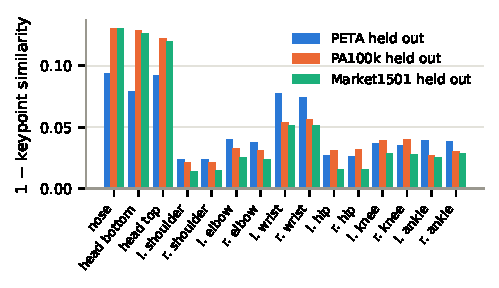
\includegraphics[width=\linewidth]{joints.pdf}
\caption{Loss of keypoint similarity per joint, $1-\exp(-d_k^2/2s^2\kappa_k^2)$ averaged over labeled instances (held-out huge models). Head points have the smallest $\kappa$.}
\label{fig:joints}
\end{figure}

%=====================================================================
\section{Hidden-Test Results}
\label{sec:test}

\begin{table}[t]
\centering\small
\setlength{\tabcolsep}{3pt}
\resizebox{\columnwidth}{!}{%
\begin{tabular}{@{}llcc@{}}
\toprule
& Changes from the previous row & LODO $\Delta$ & Test AP \\
\midrule
example & ViTPose++ S, zero-shot (organizers) & -- & 62.38 \\
v1 & ViTPose++ B, fine-tuned on two datasets & -- & 88.13 \\
v2 & ViTPose++ L, three datasets, 5 epochs & -- & 89.39 \\
v4 & huge instead of large & +0.10 & 89.58 \\
v3 & average of L and H heatmaps & +0.26 & 89.77 \\
v6 & learned score & +0.15 & \textbf{89.92} \\
\bottomrule
\end{tabular}}
\caption{Hidden-test submissions in order of the changes they make (AP $\times100$). LODO $\Delta$ is the mean held-out gain of the same change. v2 changes three factors at once.}
\label{tab:main}
\end{table}

\Cref{tab:main} lists the submissions. The fine-tuned base model v1 is the meaningful baseline; the organizers' zero-shot example suffers from the head-keypoint mismatch of \cref{sec:models}. The last three steps change one factor each, and all three agree in sign with the protocol. The learned score added 0.15\pts, inside its held-out range of 0.06 to 0.25\pts\ for the ensemble. This is consistent with the protocol representing the test domain for score changes, but it is one observation.

The deployed rescorer meets features it was not validated on. It was trained on heatmaps of two-epoch held-out models and is applied to five-epoch models trained on all data, whose heatmaps may be sharper. We verified the code path end to end, with held-out PETA models and a rescorer trained without PETA, but not this distribution shift. Absolute AP is lower on the test set (about 0.90) than on held-out datasets (about 0.93); the test images, some with several people per image, are apparently harder.

%=====================================================================
\section{Discussion}

\paragraph{What this means for design.} With one prediction per person, the order of predictions is a design target of its own. In our measurements a perfect order is worth more than a second network, and a good part of what is achievable comes from making the default score consistent with the metric, here by excluding channels the metric never scores. Beyond that, gains require telling one-pixel errors from two-pixel ones, which heatmap statistics capture only partly. The largest single error source on PETA is not the score but inversions, which neither the score nor flip testing can see.

\paragraph{Limitations.} Each configuration was trained once, and the epoch-to-epoch variation is a lower bound on training noise. Held-out models train for two epochs, submitted models for five. The shared-joint comparison was run on PETA only. The leave-one-dataset-out data have one box per image, unlike part of the test set. Our use of ViTPose++ rests on the reading of the rules stated in \cref{sec:task}.

\paragraph{Broader impact.} Pose estimation on surveillance video can support monitoring of individuals. We report technical findings only and do not release trained models.

\section{Conclusion}

When boxes are given, keypoint AP is bounded by the fraction of correct predictions and its square, and the confidence score decides where between them a system lands. On unseen surveillance cameras this is worth more than a second model, almost all of it at OKS 0.95 on two of three datasets. A learned score recovers part of it, mostly by ignoring unscored channels. The next gains are likely to come from detecting left--right inversions.

{\small
\begin{thebibliography}{99}\setlength{\itemsep}{0pt}
\bibitem{coco} T.-Y.~Lin \etal. Microsoft COCO: Common objects in context. In \textit{ECCV}, 2014.
\bibitem{posetrack} M.~Andriluka \etal. PoseTrack: A benchmark for human pose estimation and tracking. In \textit{CVPR}, 2018.
\bibitem{simplebaseline} B.~Xiao, H.~Wu, Y.~Wei. Simple baselines for human pose estimation and tracking. In \textit{ECCV}, 2018.
\bibitem{hrnet} K.~Sun, B.~Xiao, D.~Liu, J.~Wang. Deep high-resolution representation learning for human pose estimation. In \textit{CVPR}, 2019.
\bibitem{vitpose} Y.~Xu, J.~Zhang, Q.~Zhang, D.~Tao. ViTPose: Simple vision transformer baselines for human pose estimation. In \textit{NeurIPS}, 2022.
\bibitem{vitposepp} Y.~Xu, J.~Zhang, Q.~Zhang, D.~Tao. ViTPose++: Vision transformer for generic body pose estimation. \textit{IEEE TPAMI}, 2024.
\bibitem{mae} K.~He \etal. Masked autoencoders are scalable vision learners. In \textit{CVPR}, 2022.
\bibitem{udp} J.~Huang, Z.~Zhu, F.~Guo, G.~Huang. The devil is in the details: Delving into unbiased data processing for human pose estimation. In \textit{CVPR}, 2020.
\bibitem{dark} F.~Zhang, X.~Zhu, H.~Dai, M.~Ye, C.~Zhu. Distribution-aware coordinate representation for human pose estimation. In \textit{CVPR}, 2020.
\bibitem{gpose} G.~Papandreou \etal. Towards accurate multi-person pose estimation in the wild. In \textit{CVPR}, 2017.
\bibitem{ronchi} M.~R.~Ronchi, P.~Perona. Benchmarking and error diagnosis in multi-instance pose estimation. In \textit{ICCV}, 2017.
\bibitem{dekr} Z.~Geng, K.~Sun, B.~Xiao, Z.~Zhang, J.~Wang. Bottom-up human pose estimation via disentangled keypoint regression. In \textit{CVPR}, 2021.
\bibitem{ccnet} K.~Gu, R.~Chen, X.~Yu, A.~Yao. On the calibration of human pose estimation. In \textit{ICML}, 2024.
\bibitem{regda} J.~Jiang, Y.~Ji, X.~Wang, Y.~Liu, J.~Wang, M.~Long. Regressive domain adaptation for unsupervised keypoint detection. In \textit{CVPR}, 2021.
\bibitem{kim2022} D.~Kim, K.~Wang, K.~Saenko, M.~Betke, S.~Sclaroff. A unified framework for domain adaptive pose estimation. In \textit{ECCV}, 2022.
\bibitem{friedman} J.~H.~Friedman. Greedy function approximation: A gradient boosting machine. \textit{Annals of Statistics}, 2001.
\bibitem{lightgbm} G.~Ke \etal. LightGBM: A highly efficient gradient boosting decision tree. In \textit{NeurIPS}, 2017.
\end{thebibliography}
}

\clearpage
\appendix
\onecolumn
\section{Fine-tuning epochs}
\label{app:epochs}

\begin{table}[h]
\centering\small
\begin{tabular}{@{}lccccc@{}}
\toprule
PETA held out & zero-shot & epoch 1 & epoch 2 & epoch 3 & epoch 4 \\
\midrule
ViTPose++ small (4-epoch schedule) & 70.21 & 92.79 & 92.86 & 92.79 & 93.01 \\
ViTPose++ base (3-epoch schedule) & 70.90 & 93.23 & 92.97 & 93.32 & -- \\
ViTPose++ large (2-epoch schedule) & not run & 93.01 & 93.14 & -- & -- \\
ViTPose++ huge (2-epoch schedule) & 70.25 & 93.25 & 93.04 & -- & -- \\
\bottomrule
\end{tabular}
\caption{Held-out PETA AP ($\times100$) during fine-tuning. Schedules differ in length, so equal epoch numbers are at different points of the cosine schedule.}
\end{table}

\section{Implementation}

The 150 trees are stored as six $150\times13$ arrays (feature, threshold, left child, right child, leaf flag, value) plus a bias, 82\,KB in total, and evaluated with array indexing. The crop warp, Gaussian blur and DARK decoding are tensor operations, so the keypoint path runs on the GPU. Code: \texttt{pose.py} trains and evaluates a model, \texttt{rescore\_feats.py} extracts held-out features, \texttt{rescore\_eval.py} and \texttt{rescore\_ens\_eval.py} run the two-level evaluation, and \texttt{rescore\_export.py} fits the final regressor.

\end{document}
